\begin{BiliFigure}[label=figure:12][htb]{$\mathrm{LI}-\left(\sigma_{\mathrm{p}}^{\prime}/\mathrm{P}_{\mathrm{a}}\right)-S_{\mathrm{t}}$ model by \citet{Ching2012522}}{\citet{Ching2012522}提出的$\mathrm{LI}-\left(\sigma_{\mathrm{p}}^{\prime}/\mathrm{P}_{\mathrm{a}}\right)-S_{\mathrm{t}}$模型}
    \subfigure[F-CLAY/10/216]{
        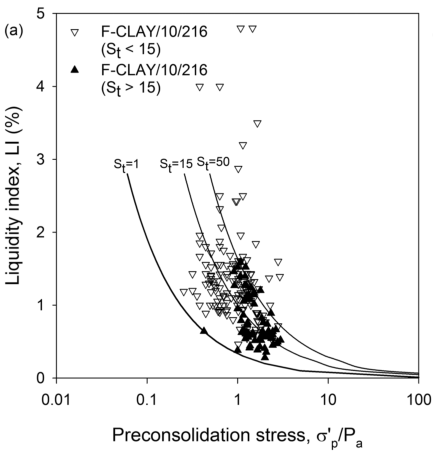
\includegraphics[width=0.48\textwidth]{figures/figure-12a.png}
        \label{figure:12a}
    }
    \hspace{\fill}
    \subfigure[S-CLAY/10/168]{
        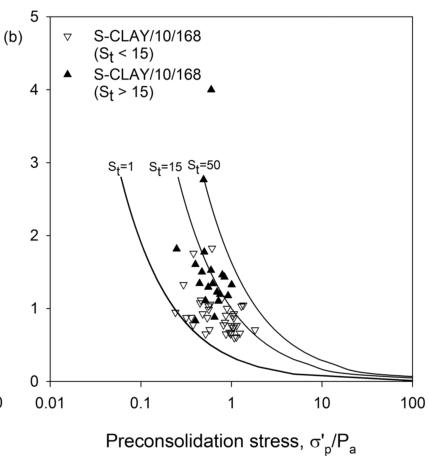
\includegraphics[width=0.48\textwidth]{figures/figure-12b.png}
        \label{figure:12b}
    }
\end{BiliFigure}